\documentclass[11pt]{amsart}
\usepackage[margin=2.6cm]{geometry}
\usepackage{amssymb,amsmath,graphicx}
\usepackage[utf8]{inputenc}
\usepackage{newunicodechar}
% characters of the Lean excerpt in Section 9
\newunicodechar{ℂ}{\ensuremath{\mathbb{C}}}
\newunicodechar{ℝ}{\ensuremath{\mathbb{R}}}
\newunicodechar{₁}{\ensuremath{_1}}
\newunicodechar{₂}{\ensuremath{_2}}
\newunicodechar{ρ}{\ensuremath{\rho}}
\newunicodechar{≤}{\ensuremath{\le}}
\newunicodechar{∧}{\ensuremath{\wedge}}
\newunicodechar{‖}{\ensuremath{\|}}
\usepackage[hidelinks]{hyperref}
\newtheorem{theorem}{Theorem}
\newtheorem{corollary}[theorem]{Corollary}
\newtheorem{lemma}[theorem]{Lemma}
\newtheorem{proposition}[theorem]{Proposition}
\theoremstyle{remark}\newtheorem{remark}[theorem]{Remark}
\theoremstyle{definition}\newtheorem{example}[theorem]{Example}
\newcommand{\C}{\mathbb{C}}
\newcommand{\Tr}{\operatorname{Tr}}
\newcommand{\Res}{\operatorname{Res}}
\newcommand{\cl}{\overline}
% VAMSHI: read every proof and reference, then delete this line.

\title{Polynomial lemniscates meet in at most $2n_1n_2-2$ points}
\author{Vamshi Jandhyala}
\date{Preprint, version 1, 8 October 2026. Not peer reviewed.}
\subjclass[2020]{30C10; 14H50; 14P05; 68V20}
\keywords{lemniscate, Cassini oval, level curves of polynomials, resultant, trace, formal verification}

\begin{document}
\begin{abstract}
Orevkov and Pakovich proved that the lemniscates $|P_1|=\rho_1$ and $|P_2|=\rho_2$ of two rational functions of
degrees $n_1,n_2$ meet in at most $2n_1n_2$ points when they meet in finitely many, that this is sharp for rational
functions, and remarked that it does not seem sharp for polynomials. We show that two polynomial lemniscates of
degrees $n_1,n_2\ge2$ with finitely many common points have at most $2n_1n_2-2$ of them. The bound is attained for
$(n_1,n_2)=(2,2)$ and $(2,3)$, so the maximum is $6$ and $10$ there; in particular two distinct Cassini ovals, and
two Bernoulli lemniscates, meet in at most six points, which answers a question from Mathematics Stack Exchange.
The proof treats $z$ and $\cl z$ as independent variables: the $2n_1n_2$ complex solutions, counted with
multiplicity, have a weighted sum that equals $-\tfrac{n_1n_2}{2}|c_1-c_2|^2\le0$ for explicit centres $c_1,c_2$,
and this forces two of them off the real locus. Every proof is formally verified in Lean.
\end{abstract}
\maketitle

\noindent\emph{Status of this preprint.} Every theorem, proposition, lemma and corollary is formally verified in
Lean~4 with Mathlib, using only Lean's standard axioms (Section~\ref{sec:lean}), except that the ten common points
in Corollary~\ref{cor:23} are certified by interval arithmetic and rechecked by an independent program. This version
has not yet been independently reviewed.

\section{Introduction}\label{sec:intro}

How many points can two lemniscates of Bernoulli have in common? The question was asked on Mathematics Stack
Exchange in 2015 \cite{mse}. A lemniscate of Bernoulli is a quartic curve with nodes at the two circular points at
infinity, so B\'ezout's theorem gives $16$ intersections in the complex projective plane, of which at least $8$ sit
at the circular points; that leaves at most $8$ real ones. Experiments suggested that $6$ is the truth, and the
asker wanted to know where the other two complex points are.

Figure~\ref{fig:six} shows six common points. The lemniscate with foci $\pm1$ is $|z^2-1|=1$, the one with foci
$0,2$ is $|(z-1)^2-1|=1$, and they cross at $z=\tfrac12\pm\tfrac i2\sqrt{4\sqrt2-5}$ and
$z=\tfrac12\pm\sqrt{2/3}\pm\tfrac{i}{\sqrt{12}}$. We prove that six is the most possible, and we prove it as
the case $n_1=n_2=2$ of a statement about all polynomial lemniscates.

\begin{figure}[ht]
\centering
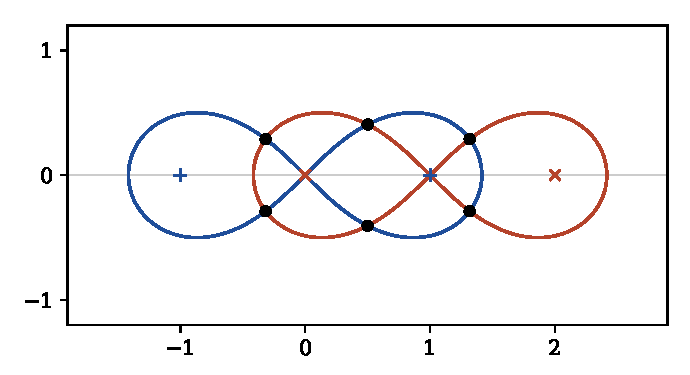
\includegraphics[width=0.62\textwidth]{figs/six.pdf}
\caption{The Bernoulli lemniscates $|z^2-1|=1$ (blue, foci $\pm1$) and $|(z-1)^2-1|=1$ (red, foci $0,2$) meet in six
points (black).}\label{fig:six}
\end{figure}

For a nonconstant rational function $P$ and $\rho>0$, the lemniscate $\{z\in\C:|P(z)|=\rho\}$ is the set of
real points of an algebraic curve of degree $2\deg P$. Orevkov and Pakovich \cite{op} proved that two such
lemniscates, of degrees $n_1$ and $n_2$, have at most $2n_1n_2$ common points when they have finitely many, and that
$2n_1n_2$ is attained by rational functions of every pair of degrees; this sharpened the bound $(n_1+n_2)^2$ of
Pakovich and Shparlinski \cite[Theorem~2.2]{ps}. For polynomials they constructed lemniscates
with $M(n_1,n_2)=n_1n_2+n_2+de$ common points, where $n_1\le n_2$, $d=\gcd(n_1,n_2)$, and $e$ is $1$ if $n_1/d$ is
even and $0$ otherwise, and they remarked that $2n_1n_2$ ``does not seem'' sharp for polynomials \cite[Section~2.5]{op}.
For $n_1=1$ (a circle) the two numbers agree, $M(1,n_2)=2n_2$. Our main result settles the remark for all other
degrees.

\begin{theorem}\label{thm:main}
Let $P_1,P_2\in\C[z]$ have degrees $n_1,n_2\ge2$, let $\rho_1,\rho_2>0$ and
$\Gamma_k=\{z\in\C:|P_k(z)|=\rho_k\}$. If $\Gamma_1\cap\Gamma_2$ is finite, then
\[
\#(\Gamma_1\cap\Gamma_2)\le 2n_1n_2-2 .
\]
\end{theorem}

\begin{corollary}\label{cor:cassini}
Two distinct Cassini ovals $|(z-a)(z-b)|=\rho$ meet in at most six points. In particular two distinct lemniscates
of Bernoulli meet in at most six points, and six is attained (Figure~\ref{fig:six}).
\end{corollary}

\begin{corollary}\label{cor:23}
The maximum number of common points of two polynomial lemniscates of degrees $2$ and $3$ with finitely many common
points is $10$, attained by $|(z-\tfrac1{10})^2-1|=1$ and $|z^3/8000-1|=1$. The pairs $(2,2)$ and $(2,3)$ are the
only ones, with $2\le n_1\le n_2$, for which $M(n_1,n_2)=2n_1n_2-2$.
\end{corollary}

\subsection*{The idea}
Write $P_k=\lambda_kf_k$ with $f_k$ monic, so that $z\in\Gamma_k$ means $f_k(z)\cl{f_k(z)}=r_k$ with
$r_k=(\rho_k/|\lambda_k|)^2$. Replace $\cl z$ by a second variable $W$ and the conjugate value $\cl{f_k(z)}$ by
$g_k(W)$, where $g_k$ has the conjugate coefficients of $f_k$. The system
\begin{equation}\label{eq:system}
f_1(Z)\,g_1(W)=r_1,\qquad f_2(Z)\,g_2(W)=r_2
\end{equation}
has, when $f_1$ and $f_2$ are coprime, exactly $2n_1n_2$ solutions $(Z,W)\in\C^2$ counted with multiplicity, and a
point $z$ lies on both lemniscates exactly when $(z,\cl z)$ is a solution. The map $\sigma(Z,W)=(\cl W,\cl Z)$
permutes the solutions, and its fixed points are the pairs $(z,\cl z)$. The heart of the proof is the identity
\begin{equation}\label{eq:identity}
\sum_{\text{solutions}}(Z-m)(W-\cl m)=-\frac{n_1n_2}{2}\,|c_1-c_2|^2 ,\qquad m=\frac{c_1+c_2}{2},
\end{equation}
where $c_k$ is the centroid of the roots of $f_k$. In words: after centring at the midpoint of the two centroids,
the weighted sum of the products $(Z-m)(W-\cl m)$ over all solutions is a real number that is never positive. A
real solution $(z,\cl z)$ contributes $|z-m|^2\ge0$. So if all solutions were real, every one of them would sit at
$z=m$; hence at least one solution is not real, and with it its partner under $\sigma$. That accounts for two of the
$2n_1n_2$ solutions and gives Theorem~\ref{thm:main} in the coprime case (Section~\ref{sec:pairing}). For the two
Bernoulli lemniscates of Figure~\ref{fig:six}, $c_1=0$, $c_2=1$, the sum is $-2$, and the two missing points the
asker looked for are the solutions $(\tfrac12\mp t,\tfrac12\pm t)$ with $t^2=\tfrac54+\sqrt2$ (Figure~\ref{fig:pair}).

\begin{figure}[ht]
\centering
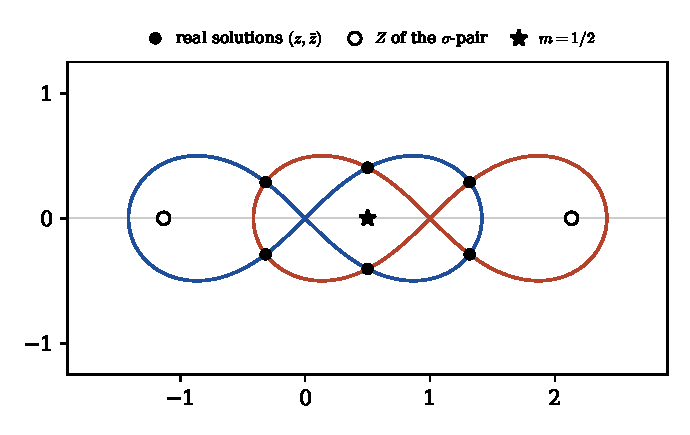
\includegraphics[width=0.62\textwidth]{figs/pairing.pdf}
\caption{The eight solutions of \eqref{eq:system} for the lemniscates of Figure~\ref{fig:six}, drawn by their
$Z$-coordinate. Six are real, $W=\cl Z$, and contribute $|Z-\tfrac12|^2$, in total $\tfrac12+2\sqrt2$. The other two
are $(\tfrac12-t,\tfrac12+t)$ and its image $(\tfrac12+t,\tfrac12-t)$ under $\sigma$, with $t^2=\tfrac54+\sqrt2$;
each contributes $(Z-\tfrac12)(W-\tfrac12)=-(\tfrac54+\sqrt2)$. The total is $-2$, as \eqref{eq:identity}
predicts.}\label{fig:pair}
\end{figure}

Identity \eqref{eq:identity} is proved by deformation. The left side is a trace (Section~\ref{sec:trace}); as the level
$r_1$ varies it is a polynomial in $r_1$ (Section~\ref{sec:deform}); the solutions grow at most like $|r_1|^{1/2}$,
so the polynomial is constant (Section~\ref{sec:growth}); and at level $0$ the algebra splits into two tensor products
whose traces are computed directly (Section~\ref{sec:level0}). A second deformation, in $r_2$, brings the second
level to $0$ as well. No intersection theory is needed: the solution count $2n_1n_2$ comes out of the same
computation at level $0$. When $f_1$ and $f_2$ share a root (Section~\ref{sec:shared}) we eliminate $W$: the
resultant $R(Z)$ vanishes at every common point, and a shared root removes its top two coefficients, so it has at
most $2n_1n_2-2$ roots unless it vanishes identically, in which case the two lemniscates turn out to be nested.

\section{Doubling the variable}\label{sec:pairing}

For $f\in\C[z]$ write $\cl f$ for the polynomial with conjugate coefficients, so that $\cl f(\cl z)=\cl{f(z)}$.
Throughout, $f_1,f_2$ are monic of degrees $n_1,n_2\ge2$, $r_1,r_2>0$, and $g_k=\cl{f_k}$. Put
\[
F_k(Z,W)=f_k(Z)\,g_k(W)-r_k\in\C[Z,W],\qquad \sigma(Z,W)=(\cl W,\cl Z).
\]
Then $F_k(z,\cl z)=|f_k(z)|^2-r_k$, so $z\in\Gamma_k$ if and only if $F_k(z,\cl z)=0$, and
$F_k(\sigma(Z,W))=f_k(\cl W)g_k(\cl Z)-r_k=\cl{F_k(Z,W)}$, so $\sigma$ maps the common zero set of $F_1,F_2$ to itself.
The fixed points of $\sigma$ are exactly the pairs $(z,\cl z)$.

The next lemma is the counting step. It says that a multiset of solutions closed under $\sigma$, with a nonpositive
weighted sum, always leaves two of its members off the real locus.

\begin{lemma}\label{lem:pairing}
Let $S$ be a finite multiset of points of $\C^2$ with $N\ge3$ members, such that $\sigma(p)$ is a member of $S$
whenever $p$ is, and let $m\in\C$ with $\sum_{p\in S}(Z_p-m)(W_p-\cl m)$ a real number $\le0$. Then at most $N-2$
distinct points of the form $(z,\cl z)$ are members of $S$.
\end{lemma}

\begin{proof}
Suppose $N-1$ distinct points $(z,\cl z)$ are members. If some member $q$ is not of this form, then $\sigma(q)\ne q$
is a member as well, also not of this form, and $q,\sigma(q)$ and the $N-1$ fixed points give $N+1$ members:
impossible. So every member has the form $(z,\cl z)$ and contributes $(z-m)\cl{(z-m)}=|z-m|^2\ge0$. The sum is then
$\ge0$, hence $0$, so every member equals $(m,\cl m)$, contradicting the $N-1\ge2$ distinct members.
\end{proof}

\section{Traces in a finite-dimensional algebra}\label{sec:trace}

To speak of the solutions of \eqref{eq:system} with multiplicity we use the quotient algebra. For a
finite-dimensional commutative $\C$-algebra $A$ and $x\in A$ write $\Tr_A(x)$ for the trace of multiplication by $x$.

\begin{lemma}\label{lem:trace}
Let $A$ be a finite-dimensional commutative $\C$-algebra and $a,b\in A$. There is a multiset $S$ of points of
$\C^2$ with $\dim A$ members such that
\begin{enumerate}
\item $\Tr_A\bigl(P(a,b)\bigr)=\sum_{p\in S}P(p)$ for every $P\in\C[Z,W]$;
\item if $P(a,b)=0$ then $P(p)=0$ for every member $p$;
\item $(\chi(a),\chi(b))$ is a member of $S$ for every $\C$-algebra map $\chi\colon A\to\C$.
\end{enumerate}
\end{lemma}

\begin{proof}
Multiplication by $a$ and by $b$ commute, so $A$ is the direct sum of the joint generalised eigenspaces
$V_\chi=\{v:(a-\chi_1)^kv=(b-\chi_2)^kv=0\text{ for some }k\}$, $\chi\in\C^2$. Let $S$ contain each $\chi$ with
multiplicity $\dim V_\chi$. Let $I_\chi$ be the radical of the annihilator of $V_\chi$, an ideal of $A$; it
contains $a-\chi_1$ and $b-\chi_2$, so $P(a,b)-P(\chi)\in I_\chi$ for every $P$. Hence $P(a,b)$ acts on $V_\chi$ as
$P(\chi)$ plus a nilpotent map, whose trace is $0$, and summing over $\chi$ gives (1); $P=1$ gives $\#S=\dim A$. If
$P(a,b)=0$ then $P(\chi)^k$ annihilates $V_\chi\ne0$, so $P(\chi)=0$: this is (2). For (3), $\chi$ vanishes on
$V_\psi$ whenever $\psi\ne(\chi(a),\chi(b))$: if $\psi_1\ne\chi(a)$, then
$(\chi(a)-\psi_1)^k\chi(v)=\chi\bigl((a-\psi_1)^kv\bigr)=0$ for $v\in V_\psi$, and if $\psi_2\ne\chi(b)$ the same holds
with $b$. Since $\chi(1)=1$ and $1$ is a sum of elements of the $V_\psi$, the space $V_{(\chi(a),\chi(b))}$ is nonzero.
\end{proof}

\section{Deforming the level}\label{sec:deform}

We now let the first level vary. Fix $G=f'(Z)g'(W)-r$ and $h=f(Z)g(W)$, and study the algebras
$\C[Z,W]/(G,h-c)$ for all $c\in\C$ at once, as the fibres of one module over $\C[t]$.

\begin{lemma}\label{lem:nocommon}
Let $f_1,f_2$ be coprime and nonconstant, and $g_1,g_2$ monic, coprime and nonconstant. For every $c\in\C$ and
$r\ne0$, the polynomials $f_1g_1-c$ and $f_2g_2-r$ have no common prime factor in $\C[Z,W]$; neither do $f_1g_1$ and
$f_2g_2-c$.
\end{lemma}

\begin{proof}
Let $H$ be a prime common factor. Suppose first that $H$ does not involve $W$. Then $H=Z-\zeta$ up to a unit, and
substituting $Z=\zeta$ in the second polynomial gives $f_2(\zeta)g_2(W)=r$ (respectively $=c$) identically in $W$.
As $g_2$ is nonconstant, $f_2(\zeta)=0$; for the first pair this contradicts $r\ne0$, and for the second pair the
first polynomial gives $f_1(\zeta)g_1(W)=0$ identically, so $f_1(\zeta)=0$, contradicting the coprimality of $f_1,f_2$.

So $H$ has positive degree in $W$. Since $g_1,g_2$ are monic, the leading coefficients in $W$ of the two polynomials
are $f_1(Z)$ and $f_2(Z)$, and the leading coefficient of $H$ divides both, so it is a constant. For the first pair
with $c\ne0$, take a root $\zeta$ of $f_1$: then $H(\zeta,W)$ still has positive degree and divides
$f_1(\zeta)g_1(W)-c=-c\ne0$, which is impossible. For the first pair with $c=0$, and for the second pair, $H$ divides
$f_1(Z)g_1(W)$, so it divides $g_1(W)$ and is $W-\omega$ up to a unit, with $g_1(\omega)=0$. Substituting $W=\omega$
in the other polynomial gives $f_2(Z)g_2(\omega)=r$ or $=c$ identically in $Z$, so $g_2(\omega)=0$ (and $r=0$ or
$c=0$); a common root of $g_1,g_2$ contradicts their coprimality, and $r=0$ contradicts $r\ne0$.
\end{proof}

The next lemma reads off the leading terms of a resultant from the leading terms of the entries. For polynomials
$P,Q$ in $W$ and integers $m\ge\deg_WP$, $n\ge\deg_WQ$, let $\Res^{m,n}(P,Q)$ be the determinant of the Sylvester
matrix of size $m+n$, with $m$ columns of shifted coefficients of $Q$ and $n$ of $P$.

\begin{lemma}\label{lem:restop}
Let $K$ be a commutative ring and $P,Q\in K[Z][W]$ with $\deg_WP\le m$, $\deg_WQ\le n$, every $W$-coefficient of
$P$ of $Z$-degree at most $d_1$ and of $Q$ at most $d_2$. Let $\hat P,\hat Q\in K[W]$ collect the coefficients of
$Z^{d_1}$ in the coefficients of $P$, and of $Z^{d_2}$ in those of $Q$. Then $\Res^{m,n}_W(P,Q)\in K[Z]$ has degree at
most $D=md_2+nd_1$, and its coefficient of $Z^{D}$ is $\Res^{m,n}(\hat P,\hat Q)$. If moreover $d_1,d_2\ge1$ and
the coefficients of $Z^{d_k-1}$ are $e_k$ times those of $Z^{d_k}$, then the coefficient of $Z^{D-1}$ is
$(me_2+ne_1)\Res^{m,n}(\hat P,\hat Q)$.
\end{lemma}

\begin{proof}
In the Leibniz expansion of the Sylvester determinant each product takes one entry from each column; the entries of
a $Q$-column have degree $\le d_2$, those of a $P$-column $\le d_1$. A product of polynomials of degrees
$\le\delta_j$ has degree $\le\sum\delta_j$, with top coefficient the product of the top coefficients, and its
coefficient of degree $\sum\delta_j-1$ is $\sum_j(\text{coefficient of degree }\delta_j-1\text{ in factor }j)\prod_{i\ne j}(\text{top of factor }i)$.
Under the proportionality assumption this is $(\sum_je_j)\prod_j(\text{top})$. Summing over permutations gives the two
claims, since the matrix of top coefficients is the Sylvester matrix of $\hat P,\hat Q$.
\end{proof}

\begin{proposition}\label{prop:deform}
Let $f,g,f',g'$ be monic of positive degree, $f,f'$ coprime, $g,g'$ coprime, $r\in\C$, and assume that for no $c$
do $h-c$ and $G$ have a common prime factor, where $h=f(Z)g(W)$ and $G=f'(Z)g'(W)-r$. Let $M=\C[Z,W]/(G)$, a
$\C[t]$-algebra by $t\mapsto h$. Then $M$ is a free $\C[t]$-module of finite rank $N$. For every $c\in\C$ the fibre
$Q_c=M/(t-c)M=\C[Z,W]/(G,h-c)$ has dimension $N$, and for every $P\in\C[Z,W]$ there is a polynomial
$\tau_P\in\C[t]$, not depending on $c$, with $\Tr_{Q_c}(P)=\tau_P(c)$.
\end{proposition}

\begin{proof}
\emph{Finite.} In $\C[t][Z][W]$ the resultant $\Res_W(f(Z)g(W)-t,\,G)$ is a combination of the two polynomials, so it
vanishes in $M$ when $t=h$. Its $W$-coefficients are $f(Z)\cdot(\text{coefficient of }g)$ minus $t$ in degree $0$,
and $f'(Z)\cdot(\text{coefficient of }g')$ minus $r$; with $d_1=\deg f\ge1$, $d_2=\deg f'$, Lemma~\ref{lem:restop}
shows that it has $Z$-degree $\deg g\deg f'+\deg g'\deg f$ with top coefficient $\Res(g,g')$, a nonzero constant
because $g,g'$ are coprime. Dividing by it, $Z$ is a root of a monic polynomial over $\C[t]$; exchanging the roles
of $Z$ and $W$ (using that $f,f'$ are coprime) does the same for $W$. As $M$ is generated by $Z$ and $W$, it is a
finite $\C[t]$-module.

\emph{Torsion-free.} Let $p\ne0$ and $p(h)a\in(G)$. Factor $p=\lambda\prod_j(t-c_j)$. A prime factor of $G$ that
divided $p(h)=\lambda\prod_j(h-c_j)$ would divide some $h-c_j$, which is excluded, so $G$ divides $a$.

\emph{Free.} A finite torsion-free module over the principal ideal domain $\C[t]$ is free.

\emph{Fibres.} Let $b_1,\dots,b_N$ be a $\C[t]$-basis of $M$ and write $s=\sum_i\beta_i(s)b_i$ with
$\beta_i(s)\in\C[t]$. The map $s\mapsto(\beta_i(s)(c))_i$ vanishes on $(t-c)M$, and
$s-\sum_i\beta_i(s)(c)\,b_i=\sum_i\bigl(\beta_i(s)-\beta_i(s)(c)\bigr)b_i$ lies in $(t-c)M$ because $t-c$ divides
$\beta-\beta(c)$. So the images of the $b_i$ form a $\C$-basis of $Q_c$, and the matrix of multiplication by $P$ on
$Q_c$ in this basis is the matrix on $M$ with $t$ replaced by $c$. Hence $\Tr_{Q_c}(P)=\tau_P(c)$, where $\tau_P$ is
the trace over $\C[t]$ of multiplication by $P$ on $M$.
\end{proof}

Combining Proposition~\ref{prop:deform} with Lemma~\ref{lem:trace}, applied to $A=Q_c$, $a=Z$, $b=W$: \emph{for each
$c$ there is a multiset $S_c$ of $N$ common zeros of $h-c$ and $G$, containing each common zero at least once, with
$\sum_{p\in S_c}P(p)=\tau_P(c)$.} The common zeros give algebra maps $Q_c\to\C$, hence members, by
Lemma~\ref{lem:trace}(3).

\section{Growth}\label{sec:growth}

A polynomial $\tau$ in one variable with $|\tau(c)|\le A+B|c|^{1/2}$ for all $c$ is constant, since a polynomial of
degree $d\ge1$ satisfies $|\tau(c)|\ge\tfrac12|\mathrm{lc}(\tau)|\,|c|^d$ for large $|c|$. So $\tau_P(c)$ is
constant as soon as the members of $S_c$ grow at most like $|c|^{1/2}$, which is what the next lemma provides.

\begin{lemma}\label{lem:growth}
Let $\varphi=(Z-m)(W-m')$ with $m,m'\in\C$.
\begin{enumerate}
\item Let $f,g,f',g'$ be monic with $\deg f,\deg g\ge2$ and $\deg f',\deg g'\ge1$, with $f,f'$ coprime and
$g,g'$ coprime, and $r\in\C$. There are $A,B$ such that every common zero of $f(Z)g(W)-c$ and $f'(Z)g'(W)-r$ satisfies
$|\varphi|\le A+B|c|^{1/2}$, for every $c$.
\item Let $f_1,g_1,f_2,g_2$ be monic, with $\deg f_1\ge1$, $\deg g_1\ge1$, $\deg f_2\ge2$ and $\deg g_2\ge2$, and
with $f_1,f_2$ coprime and $g_1,g_2$ coprime. There are $A,B$ such that every common zero of $f_1(Z)g_1(W)$ and
$f_2(Z)g_2(W)-d$ satisfies $|\varphi|\le A+B|d|^{1/2}$, for every $d$.
\end{enumerate}
\end{lemma}

\begin{proof}
Two facts are used. A monic polynomial $u$ of degree $n\ge1$ satisfies $\tfrac12|w|^n\le|u(w)|\le2|w|^n$ once $|w|$
exceeds a constant. Coprime $p,q$ are not simultaneously small on a disc: from $up+vq=1$ and bounds for $|u|,|v|$ on
the disc, $\max(|p|,|q|)\ge\delta>0$ there.

The main step is a one-sided bound for (1): if $|W|\le R_0$ then $|Z|\le A'+B'|c|^{1/2}$. Indeed, for $|Z|$ large,
$|f'(Z)|\ge|Z|/2$, so $|g'(W)|=|r|/|f'(Z)|<\delta$, where $\delta$ is the constant for $g',g$ on the disc
$|W|\le R_0$; hence $|g(W)|\ge\delta$, and $|c|=|f(Z)|\,|g(W)|\ge\tfrac12|Z|^2\delta$ because $\deg f\ge2$. The
roles of $Z,W$ are symmetric, and $|Z|,|W|$ cannot both be large, since then $|f'(Z)g'(W)|>|r|$. So one coordinate is
bounded and the other is $O(1+|c|^{1/2})$, which bounds $|\varphi|\le(|Z|+|m|)(|W|+|m'|)$.

For (2), $f_1(Z)g_1(W)=0$ means that $Z$ is a root of $f_1$ or $W$ is a root of $g_1$, so one coordinate is bounded,
and the one-sided bound applies with $(f,g,f',g',r)=(f_2,g_2,f_1,g_1,0)$ or its mirror image.
\end{proof}

\section{Level zero and the trace identity}\label{sec:level0}

At level $0$ the algebra splits. Write $s_p$ for the sum of the roots of a monic polynomial $p$ (with multiplicity),
so $s_p=-(\text{coefficient of }z^{\deg p-1})$.

\begin{lemma}\label{lem:level0}
Let $f,f',g,g'$ be monic of positive degree with $f,f'$ coprime and $g,g'$ coprime. Then
\[
\C[Z,W]/\bigl(f(Z)g(W),\,f'(Z)g'(W)\bigr)\;\cong\;\C[Z,W]/(f',g)\times\C[Z,W]/(f,g')
\]
and $\C[Z,W]/(f,g)\cong\C[Z]/(f)\otimes\C[W]/(g)$.
Hence the algebra has dimension $\deg f'\deg g+\deg f\deg g'$, and for $\varphi=(Z-m)(W-m')$
\[
\Tr(\varphi)=(s_{f'}-m\deg f')(s_g-m'\deg g)+(s_f-m\deg f)(s_{g'}-m'\deg g').
\]
In words: each of the two factors contributes the product of its two centred root sums.
\end{lemma}

\begin{proof}
The map to the product is surjective: if $uf+vf'=1$, the element $u(Z)f(Z)$ is $1$ modulo $(f',g)$ and $0$ modulo
$(f,g')$. It is injective because $(f',g)\cap(f,g')=(f',g)(f,g')$ (the two ideals are comaximal: $f$ and $f'$
generate the unit ideal) and the four products lie in $(fg,f'g')$: $f'g'$ and $fg$ are the generators, and, with
$\tilde ug+\tilde vg'=1$,
\[
ff'=(\tilde uf')\,fg+(\tilde vf)\,f'g',\qquad gg'=(ug')\,fg+(vg)\,f'g'.
\]
The tensor isomorphism sends $Z,W$ to $Z\otimes1,1\otimes W$. Dimensions add over products and multiply over tensor
products. So do traces, and $\varphi$ is the pure tensor $(Z-m)\otimes(W-m')$ in each factor. Finally, the trace of
$Z$ on $\C[Z]/(f)$ is $s_f$ (its characteristic polynomial is $f$), so the trace of $Z-m$ is $s_f-m\deg f$.
\end{proof}

\begin{proposition}\label{prop:identity}
Let $f_1,f_2$ be coprime and $g_1,g_2$ coprime, all monic of degree at least $2$, and $r_2\ne0$. The solutions of
$f_1(Z)g_1(W)=r_1$, $f_2(Z)g_2(W)=r_2$ are the members of a multiset $S$ with $\deg f_1\deg g_2+\deg f_2\deg g_1$
members, each solution occurring at least once, and
\[
\sum_{p\in S}(Z_p-m)(W_p-m')=(s_{f_1}-m\deg f_1)(s_{g_2}-m'\deg g_2)+(s_{f_2}-m\deg f_2)(s_{g_1}-m'\deg g_1).
\]
That is, the sum over the solutions at levels $(r_1,r_2)$ equals the trace of Lemma~\ref{lem:level0} at levels
$(0,0)$.
\end{proposition}

\begin{proof}
Apply Proposition~\ref{prop:deform} to $h=f_1g_1$, $G=f_2g_2-r_2$ (Lemma~\ref{lem:nocommon} gives the hypothesis),
and let $S=S_{r_1}$, with sum $\tau_1(r_1)$. By Lemma~\ref{lem:growth}(1), $|\tau_1(c)|\le N(A+B|c|^{1/2})$, so
$\tau_1$ is constant and $\tau_1(r_1)=\tau_1(0)$, the trace on $\C[Z,W]/(f_2g_2-r_2,\,f_1g_1)$. This algebra is
also the fibre at $r_2$ of the second deformation $h=f_2g_2$, $G=f_1g_1$ (Lemma~\ref{lem:nocommon}, second part),
so the trace equals $\tau_2(r_2)$, which by Lemma~\ref{lem:growth}(2) equals $\tau_2(0)$, the trace at level
$(0,0)$, given by Lemma~\ref{lem:level0}. The number of members follows the same chain: both ranks equal the
dimension of the common fibre, and the second rank is the dimension at level $(0,0)$.
\end{proof}

\begin{proof}[Proof of Theorem~\ref{thm:main} when $f_1,f_2$ are coprime]
Take $g_k=\cl{f_k}$; then $\deg g_k=n_k$, $s_{g_k}=\cl{s_{f_k}}$, and $g_1,g_2$ are coprime. Let $c_k=s_{f_k}/n_k$ be
the centroid of the roots of $f_k$, $m=\tfrac12(c_1+c_2)$ and $m'=\cl m$. Then $s_{f_1}-mn_1=\tfrac{n_1}2(c_1-c_2)$
and $s_{f_2}-mn_2=-\tfrac{n_2}2(c_1-c_2)$, and Proposition~\ref{prop:identity} gives a multiset $S$ of
$N=2n_1n_2$ solutions with
\[
\sum_{p\in S}(Z_p-m)(W_p-\cl m)=\frac{n_1n_2}{4}(c_1-c_2)\cl{(c_2-c_1)}+\frac{n_1n_2}{4}(c_2-c_1)\cl{(c_1-c_2)}
=-\frac{n_1n_2}{2}|c_1-c_2|^2\le0 .
\]
The two terms are equal, each being $-\tfrac{n_1n_2}{4}|c_1-c_2|^2$, because $(c_1-c_2)\cl{(c_2-c_1)}=-|c_1-c_2|^2$.
Since $\sigma$ maps solutions to solutions and every solution is a member of $S$, Lemma~\ref{lem:pairing} applies
and at most $2n_1n_2-2$ points $(z,\cl z)$ are solutions. These are the common points of the lemniscates. No
finiteness assumption was used in this case.
\end{proof}

\section{Shared roots}\label{sec:shared}

Suppose $f_1$ and $f_2$ have a common root $\zeta$. We eliminate $W$: let $R(Z)=\Res^{n_1,n_2}_W(F_1,F_2)$.

\begin{lemma}\label{lem:R}
\begin{enumerate}
\item If $F_1(z,w)=F_2(z,w)=0$ then $R(z)=0$. In particular every common point $z$ of the lemniscates is a root of
$R$.
\item $\deg R\le 2n_1n_2-2$.
\end{enumerate}
\end{lemma}

\begin{proof}
(1) The resultant commutes with substituting $Z=z$, and $R(z)=p\,F_1(z,\cdot)+q\,F_2(z,\cdot)$ for polynomials $p,q$
in $W$; evaluate at $W=w$. (2) The $W$-coefficients of $F_k$ are $f_k(Z)$ times the coefficients of $g_k$, minus
$r_k$ in degree $0$. Their $Z^{n_k}$-coefficients are the coefficients of $g_k$ and, since $n_k\ge2$, their
$Z^{n_k-1}$-coefficients are $e_k$ times those, $e_k$ being the subleading coefficient of $f_k$. By
Lemma~\ref{lem:restop}, the coefficients of $Z^{2n_1n_2}$ and $Z^{2n_1n_2-1}$ in $R$ are multiples of
$\Res(g_1,g_2)$, and $\deg R\le2n_1n_2$. Since $g_1(\cl\zeta)=g_2(\cl\zeta)=0$, part (1) applied to $g_1,g_2$ (a
B\'ezout relation evaluated at a common root) gives $\Res(g_1,g_2)=0$.
\end{proof}

If $R\ne0$, distinct common points are distinct roots of $R$, and Theorem~\ref{thm:main} follows from
Lemma~\ref{lem:R}. It remains to see what $R\equiv0$ means.

\begin{lemma}\label{lem:nested}
If $R\equiv0$ then $f_1^{n_2}=f_2^{n_1}$.
\end{lemma}

\begin{proof}
For $Z$ with $f_1(Z)f_2(Z)\ne0$, the polynomials $F_1(Z,\cdot)$ and $F_2(Z,\cdot)$ have exact degrees $n_1,n_2$ and
resultant $R(Z)=0$, so they have a common root $w$. Let $\zeta$ be a root of $f_1f_2$, of multiplicity $a$ in $f_1$
and $b$ in $f_2$. As $Z\to\zeta$, one of $|g_1(w)|=r_1/|f_1(Z)|$ and $|g_2(w)|=r_2/|f_2(Z)|$ tends to infinity, so
$|w|\to\infty$, and the two-sided bounds $\tfrac12|w|^{n}\le|g_k(w)|\le2|w|^{n}$ give
$|g_1(w)|^{n_2}\asymp|w|^{n_1n_2}\asymp|g_2(w)|^{n_1}$ with constants independent of $Z$. Thus
$|f_2(Z)|^{n_1}\asymp|f_1(Z)|^{n_2}$ near $\zeta$. Along $Z=\zeta+t$, $t\to0^+$, the left side is
$\asymp t^{bn_1}$ and the right side $\asymp t^{an_2}$, so $an_2=bn_1$. Hence the monic polynomials
$f_1^{n_2}$ and $f_2^{n_1}$ have the same roots with the same multiplicities, and are equal.
\end{proof}

Compare the exceptional configurations in \cite[Theorem~2.2]{ps} and \cite[Theorem~1.1]{op}: there too the
obstruction to a finite count is that the two functions are built from a common one.

\begin{proof}[Proof of Theorem~\ref{thm:main} when $f_1,f_2$ share a root]
If $R\ne0$ we are done. If $R\equiv0$, Lemma~\ref{lem:nested} gives $|f_2|^{2n_1}=|f_1|^{2n_2}$ on $\C$. If the
lemniscates had a common point $z_0$, then $r_2^{n_1}=r_1^{n_2}$, and every $z\in\Gamma_1$ would satisfy
$|f_2(z)|^{2n_1}=r_1^{n_2}=r_2^{n_1}$, that is $z\in\Gamma_2$. But $\Gamma_1$ is infinite: at a root $\zeta$ of $f_1$
and for each small real $x$, $|f_1|^2$ is below $r_1$ at $\zeta+x$ and above it at $\zeta+x+iY$ for large $Y$, so by
the intermediate value theorem $\Gamma_1$ has a point with real part $\operatorname{Re}\zeta+x$. This contradicts
finiteness, so $\Gamma_1\cap\Gamma_2$ is empty.
\end{proof}

\section{Degree two and sharpness}\label{sec:sharp}

\begin{proof}[Proof of Corollary~\ref{cor:cassini}]
A Cassini oval is $|f(z)|=\rho$ with $f=(z-a)(z-b)$ monic of degree $2$. In the coprime case and in the case
$R\ne0$ the proof above gives at most $6$ points without assuming finiteness. If $R\equiv0$ then $f_1^2=f_2^2$, so
$(f_1-f_2)(f_1+f_2)=0$ and $f_1=f_2$, as $f_1+f_2$ has leading coefficient $2$; two ovals with the same foci and a
common point have the same level, so they are equal. The six points of Figure~\ref{fig:six} lie on both curves:
substituting them into $(x^2+y^2)^2=2(x^2-y^2)$ and its translate by $1$ is an identity in $\sqrt2$.
\end{proof}

\begin{proof}[Proof of Corollary~\ref{cor:23}]
For $f_1=(z-\tfrac1{10})^2-1$ and $f_2=z^3/8000-1$, interval arithmetic certifies ten pairwise disjoint boxes, each
containing exactly one common point of $|f_1|=1$ and $|f_2|=1$ (Section~\ref{sec:lean}); Theorem~\ref{thm:main} gives
at most $2\cdot2\cdot3-2=10$. This is the construction of \cite[Proposition~2]{op} with explicit parameters. For the
second claim, $M(n_1,n_2)=2n_1n_2-2$ means $n_2(n_1-1)=de+2\le n_1+2$. As $n_2\ge n_1$, this forces
$n_1(n_1-1)\le n_1+2$, so $n_1=2$; then $n_2=de+2$, which is $3$ for odd $n_2$ ($d=1$, $e=1$) and $2$ for even $n_2$
($d=2$, $e=0$).
\end{proof}

\begin{remark}
For other degrees the maximum lies between $M(n_1,n_2)$ and $2n_1n_2-2$, and we do not know where. The smallest open
cases are $(2,4)$, with $M(2,4)=12$ against our bound $14$, and $(3,3)$, with $M(3,3)=12$ against $16$.
\end{remark}

\section{Formal verification and data}\label{sec:lean}

Every statement above, including Corollaries~\ref{cor:cassini} and~\ref{cor:23} except the numerical certificate for
the ten points, is proved in Lean~4 with Mathlib \cite{lean,mathlib}, in about $3{,}100$ lines that depend only on
Lean's three standard axioms (propositional extensionality, choice and quotient soundness). The formal proof follows
the text, with one difference: the constancy of the trace polynomial in Section~\ref{sec:growth} is derived from
Liouville's theorem rather than from the degree argument given there. The other steps are formalised as written: joint generalised eigenspaces for Lemma~\ref{lem:trace}; the Sylvester expansion for
Lemma~\ref{lem:restop}; an explicit basis of the fibres for Proposition~\ref{prop:deform}; the Chinese remainder
theorem and tensor products for Lemma~\ref{lem:level0}; and Lemmas~\ref{lem:R} and~\ref{lem:nested} for shared
roots. The main statement reads
\begin{small}\begin{verbatim}
theorem theoremA (P₁ P₂ : ℂ[X]) (hn₁ : 2 ≤ P₁.natDegree) (hn₂ : 2 ≤ P₂.natDegree)
    {ρ₁ ρ₂ : ℝ} (hρ₁ : 0 < ρ₁) (hρ₂ : 0 < ρ₂)
    (hfin : {z : ℂ | ‖P₁.eval z‖ = ρ₁ ∧ ‖P₂.eval z‖ = ρ₂}.Finite) :
    hfin.toFinset.card ≤ 2 * P₁.natDegree * P₂.natDegree - 2
\end{verbatim}\end{small}
The corollaries are \texttt{oval\_le\_six}, \texttt{bernoulli\_six} and \texttt{M\_eq\_iff}. A mutation test plants
$19$ wrong variants (bounds off by one, wrong signs, dropped hypotheses) and checks that each is rejected. The ten points of Corollary~\ref{cor:23} and the six of Corollary~\ref{cor:cassini} are certified by
the Krawczyk test in interval arithmetic; an independent program recomputes all $2n_1n_2$ complex solutions of both
examples from an exact resultant and confirms the counts, identity \eqref{eq:identity} and the numbers in
Figure~\ref{fig:pair}. A symbolic computation confirms \eqref{eq:identity} for $n_1=n_2=2$ with all coefficients and
levels as free variables. The Lean sources, these programs and their outputs are in the folder
\texttt{polynomial-lemniscates} of \url{https://github.com/jvvk/mathematics}.

\section*{Acknowledgement}
The proofs, text, verification programs and Lean formalisation were developed with the AI assistant Claude
(Anthropic; Claude Opus 5.5 in Claude Code), under the author's direction. The author is responsible for the contents.

\begin{thebibliography}{9}

\bibitem{lean} L.~de Moura and S.~Ullrich, The Lean~4 theorem prover and programming language, in \emph{Automated
Deduction, CADE~28}, Lecture Notes in Comput. Sci.~12699, Springer, 2021, 625--635.
\url{https://doi.org/10.1007/978-3-030-79876-5_37}
\bibitem{mathlib} The mathlib Community, The Lean mathematical library, in \emph{Proceedings of the 9th ACM SIGPLAN
International Conference on Certified Programs and Proofs (CPP 2020)}, ACM, 2020, 367--381.
\url{https://doi.org/10.1145/3372885.3373824}
\bibitem{mse} Mostafa, Maximum number of intersection points of two different Bernoulli lemniscates, Mathematics
Stack Exchange question 1250327, 24 April 2015. \url{https://math.stackexchange.com/q/1250327} (accessed 8 October
2026).
\bibitem{op} S.~Orevkov and F.~Pakovich, On intersection of lemniscates of rational functions, \emph{Arnold Math. J.}
\textbf{11} (2025), no.~1, 7--26. \url{https://doi.org/10.56994/ARMJ.011.001.002}
\bibitem{ps} F.~Pakovich and I.~E.~Shparlinski, Level curves of rational functions and unimodular points on rational
curves, \emph{Proc. Amer. Math. Soc.} \textbf{148} (2020), no.~5, 1829--1833.
\url{https://doi.org/10.1090/proc/14928}
\end{thebibliography}
\end{document}
